\subsection{Task 7: Triangle Counting}
According to the algorithms in \cite{}, we know that the number of triangles in a network is propotional to the sum of eigenvalue of its adjency matrix, which is $\frac{\sum_{i}\lambda_{i}^{3}}{6}$. Figure \ref{t7:time} shows the running time of global triangle counting with regards to the size of graph. We can see that as the size of graph increases, the running time also grows nearly linearly with the size. For the largest graph, which is Roadnet-PA, it runs nearly for an hour to complete. However, the predicted result for Roadnet-PA is unsatisfactory. 

\subsubsection{Plots and Statistics(Global)}

\begin{tabular}{ | c | c | }
    \hline
    graph size & run time(seconds) \\ \hline
    7115 & 45.199s \\ \hline
    36692 & 72.76 \\ \hline
    82168 & 596.046 \\ \hline
    334863 & 1288.703 \\ \hline
    1088092 & 2980.985 \\ \hline
\end{tabular}

\begin{tabular} {| c | c | c | c | }
    \hline
    dataset & size & predict & truth \\ \hline
    wiki-Vite & 7115 & 661282 & 608389 \\ \hline
    Enron-email & 36692 & 276757 & 727044 \\ \hline
    slash-dot & 82168 & 1294037 & 602592 \\ \hline
    Amazon-com & 334863 & 13904 & 667129 \\ \hline
    Roadnet-PA & 1088092 & 55.95 & 67150 \\ \hline
\end{tabular}

\begin{figure}[h]
\begin{center}
\begin{tabular}{c}
     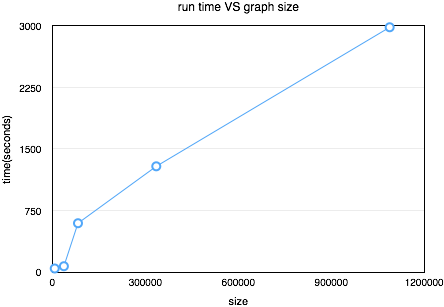
\includegraphics[width=0.8\textwidth]{FIG/t7_time.png}
\end{tabular}
\caption{Run time VS graph size(global)}
\label{t7:time}
\end{center}
\end{figure}

\subsubsection{Plots and Statistics(Local)}
\begin{figure}[h]
\begin{center}
\begin{tabular}{cc}
     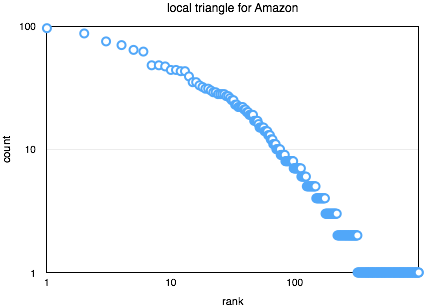
\includegraphics[width=0.4\textwidth]{FIG/t7_amazon.png} &
     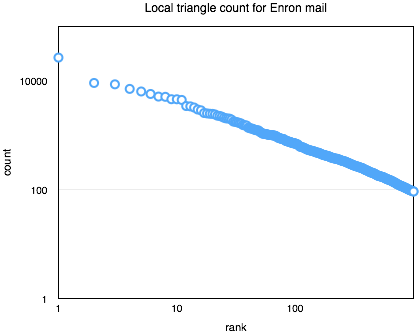
\includegraphics[width=0.4\textwidth]{FIG/t7_enron.png} \\
     (a) & (b) \\
     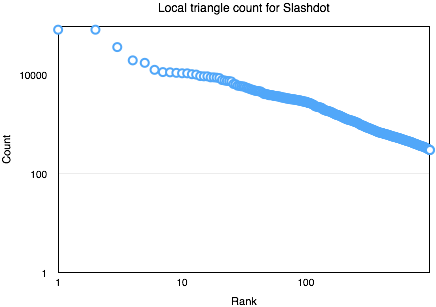
\includegraphics[width=0.4\textwidth]{FIG/t7_slashdot.png} &
     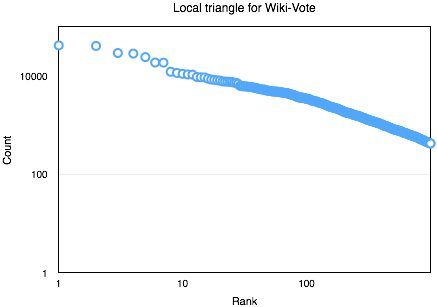
\includegraphics[width=0.4\textwidth]{FIG/t7_wikivote.png} \\
     (c) & (d) \\
     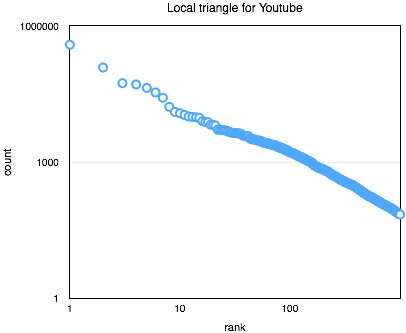
\includegraphics[width=0.4\textwidth]{FIG/t7_youtube.png} & \\
     (e)
\end{tabular}
\caption{(a) Amazon (b) Enron Mail (c) Slashdot (d) Wiki Vote (e) Youtube}
\label{t7:1}
\end{center}
\end{figure}